 
%\documentclass[review]{elsarticle}
\documentclass[final,twocolumn]{elsarticle}
%\documentclass[final,5p,times,twocolumn]{elsarticle}

\usepackage{project}

%! Author = sbbfti
%! Date = 10/06/2020

\newacronym{ADF}{ADF test}{Augmented Dickey-Fuller test}
\newacronym{KPSS}{KPSS test}{Kwiatkowski-Phillips-Schmidt-Shin test}
\newacronym{ACF}{ACF}{AutoCorrelation function}
\newacronym{PACF}{PACF}{Partial AutoCorrelation function}


\newacronym{ti}{$T_{i}$}{indoor air temperature, $^{\circ}$C}


\begin{document}

    \begin{frontmatter}
%
\title{\Huge EE6563 Project Progress\\ Footprint Recognition based on the\\ Spatio-Temporal Features }


%% Group authors per affiliation:
\author{Saeed Kazemi\fnref{myfootnote}}
\address{University of New Brunswick}
\fntext[myfootnote]{Saeed.Kazemi@unb.ca.}

%% or include affiliations in footnotes:
%\ead[url]{https://github.com/SKazemii/EE6563}

\begin{abstract}
Given present-day security concerns, many buildings have implemented robust authentication techniques. Aside from authentication to enter a building, applications such as border and airport security also administer identification. Therefore, many cities and companies provide technologies like CCTV or fingerprinting for authentication and verification. But each system has its own drawbacks. For example, due to the Covid-19 pandemic, most people wear a mask and avoid touching unnecessary surfaces. Thus, gait recognition could be a solution. 



%In this project, we worked on temporal information of time-series data. These features used to construct a classifier. Moreover, verification mode was used for this research.

%This aids to disguise people and reduces the hygiene of fingerprint biometrics respectively. In this research, we focus on which classifier has better results on barefoot footprints and which features have the important effect on the classifier.



In this paper, we present a review of the time series approaches for classification tasks including conventional machine learning algorithm and Deep Neural Networks. Also in \ref{appendix:2}, more approaches have been reviewed for classification. These approaches are implemented on verification mode. Experimental results show that SVM classifier on the contribution of all handcrafted features had the best performance with 91.3\%.

%Convolutional Neural Networks (CNN) has achieved a great success in image recognition task by automaticallylearning a hierarchical feature representation from raw data. While the majority of Time-Series Classification(TSC) literature is focused on 1D signals, this paper uses Recurrence Plots (RP) to transform time-series into2D texture images and then take advantage of the deep CNN classifier.  Image representation of time-seriesintroduces different feature types that are not available for 1D signals, and therefore TSC can be treated astexture image recognition task. CNN model also allows learning different levels of representations together witha classifier, jointly and automatically. Therefore, using RP and CNN ina unified framework is expected to boostthe recognition rate of TSC. Experimental results on the UCR time-series classification archive demonstratecompetitive accuracy of the proposed approach, compared not only to the existing deep architectures, but alsoto the state-of-the art TSC algorithms.


\end{abstract}

\begin{keyword}
Footprint recognition\sep Time series\sep pressure sensor
\end{keyword}

\end{frontmatter}


    \section{Introduction}

Contemporary security identification has led to a plethora of biometric-based authentication systems. From palm readers at testing centers to facial recognition on smartphones, many systems are now used to regularly verify identities. These inherence-based systems are attractive in comparison to knowledge or possession-based methods of authentication because biometrics are unique, unforgettable, and far more difficult to steal than a password or swipe card.

Although biometric identification appears sophisticated when compared to something like physical keys, it does not come without its own share of caveats. For example, owing to the ongoing Covid19 pandemic, many people wear masks when outside of their house, challenging most facial recognition systems. Additionally, biometrics that rely on touch, such as fingerprinting, raise safety concerns, as the scanner may become a vector for virus transmission. Despite these setbacks, given their merits and widespread deployment, biometric identification systems are unlikely to disappear.

One behavioral biometric that has gained recent success and is worth further consideration given current constraints is gait recognition. Usage of gait recognition has grown in the security industry in recent decades due to advances in deep learning. Singh et al. \cite{Singh2019APerspectives} categorized gait recognition into two main categories, vision-based and sensor-based. In vision-based approaches, cameras capture data of a person walking for the purpose of gait recognition. Sensor-based gait recognition is performed using either wearable sensors which produce kinematic data, or floor sensors which produce kinetic data \cite{Connor2018BiometricFeatures}.


********There is a big jump in thought between these two paragraphs.  Try to lead from one to the next smoothly.

%\section{Datasets}
The dataset that was used for this project is called the Stepscan dataset \cite{Connor2015ComparingBiometrics}. This dataset was obtained from high-resolution floor tiles that have recently been introduced by Stepscan Technologies Inc. Furthermore, this dataset consists of a spatial-temporal tensor, X, with dimensions $S \times T \times H \times W$ where $S$ represents the number of samples. $T$ is the number of temporal observations or video frames; $H$ and $W$ are the dimension of the image in pixels. Figure \ref{fig:Stepscan_dataset} indicates three frames from one of samples in the dataset.  

******There's another jump here. 

In general, there are two modes for footprint recognition or generally in the biometric system: verification or identification mode \cite{Jain2004AnRecognition}. In verification mode, the biometric system is used for accessing buildings or data. In other words, the system compares the claimed person with its dataset to determine whether or not the claim is valid. These systems not only consume less processing power and time but also have better performance regarding identification systems \cite{Jain2004AnRecognition}. This project aims to find some features from the datasets to construct a classifier for verification purposes. 

*******Is this really the main benefit?  What else can you think of?  What about performance/scaling?


%Because verification systems only need to compare the presented biometric to a biometric reference stored in the system, they can generate results more quickly and are more accurate than identification systems, even when the size of the database increases.

 

The rest of this paper is organized as follows: Section 2 provides the relevant works and researches. Then,% in Section 3, the time domain features as well as machine learning models are defined. In Section 4, we discuss the results, and we propose future work in Section 5.
 the classification method based on machine learning and deep learning is presented in Section 3. Also a brief survey on time series classification and Deep learning has been discussed in \ref{appendix:2}. The results and discussion are described in Sections 4 and 5.
%As the figure \ref{fig:Stepscan_dataset} shows the data is a image not a time series data. Therefore, we need to convert our data to a time series. 
Furthermore, this research will be implemented in Python, and the source codes are available on the GitHub repository \cite{SKazemii/EE6563}. 

\begin{figure}
    \centering
    \begin{minipage}[b]{.5\textwidth}
        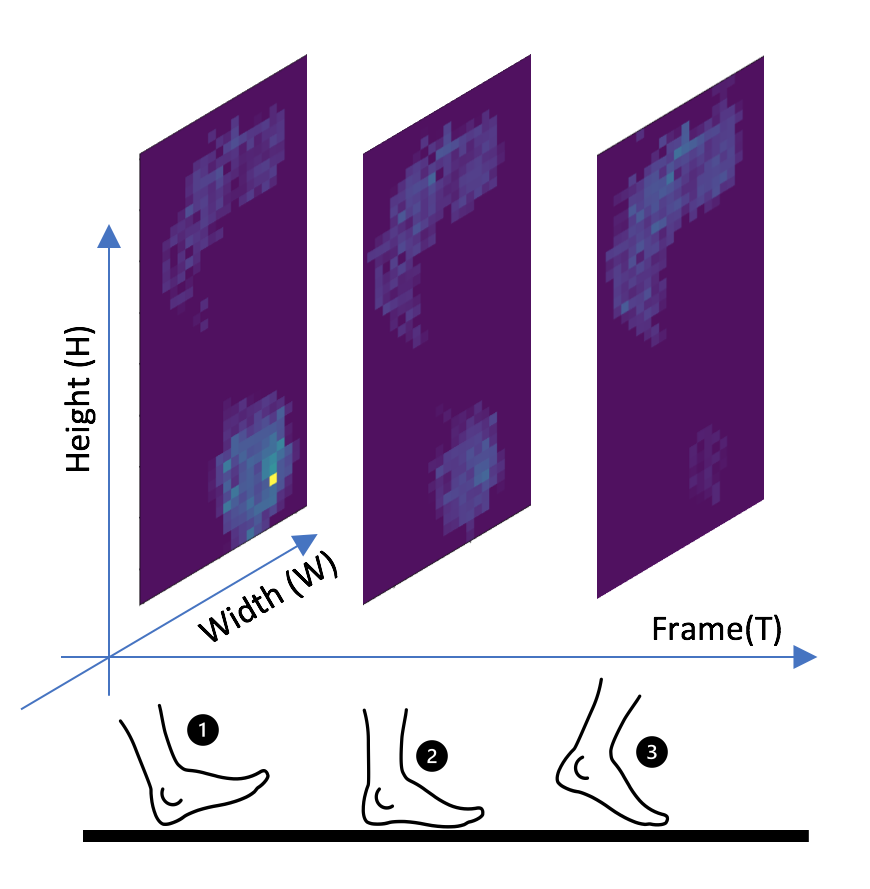
\includegraphics[width=\textwidth]{figures/project/frame2.png}
    \end{minipage}
    \caption{Different frames of footprint video in Stepscan dataset.}
    \label{fig:Stepscan_dataset}
\end{figure}


\begin{figure}
     \centering
     \begin{subfigure}[b]{0.5\textwidth}
         \centering
         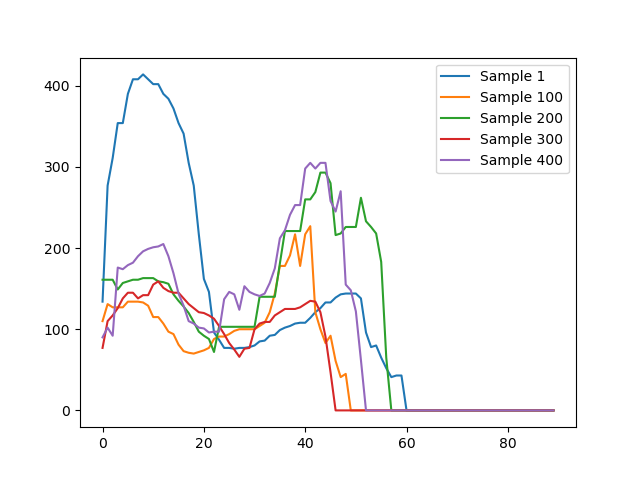
\includegraphics[width=0.9\textwidth]{figures/project/df_max.png}
         \caption{The maximum pressure in each frame}
         \label{fig:extracted_features_max}
     \end{subfigure}
     \hfill
     \begin{subfigure}[b]{0.5\textwidth}
         \centering
         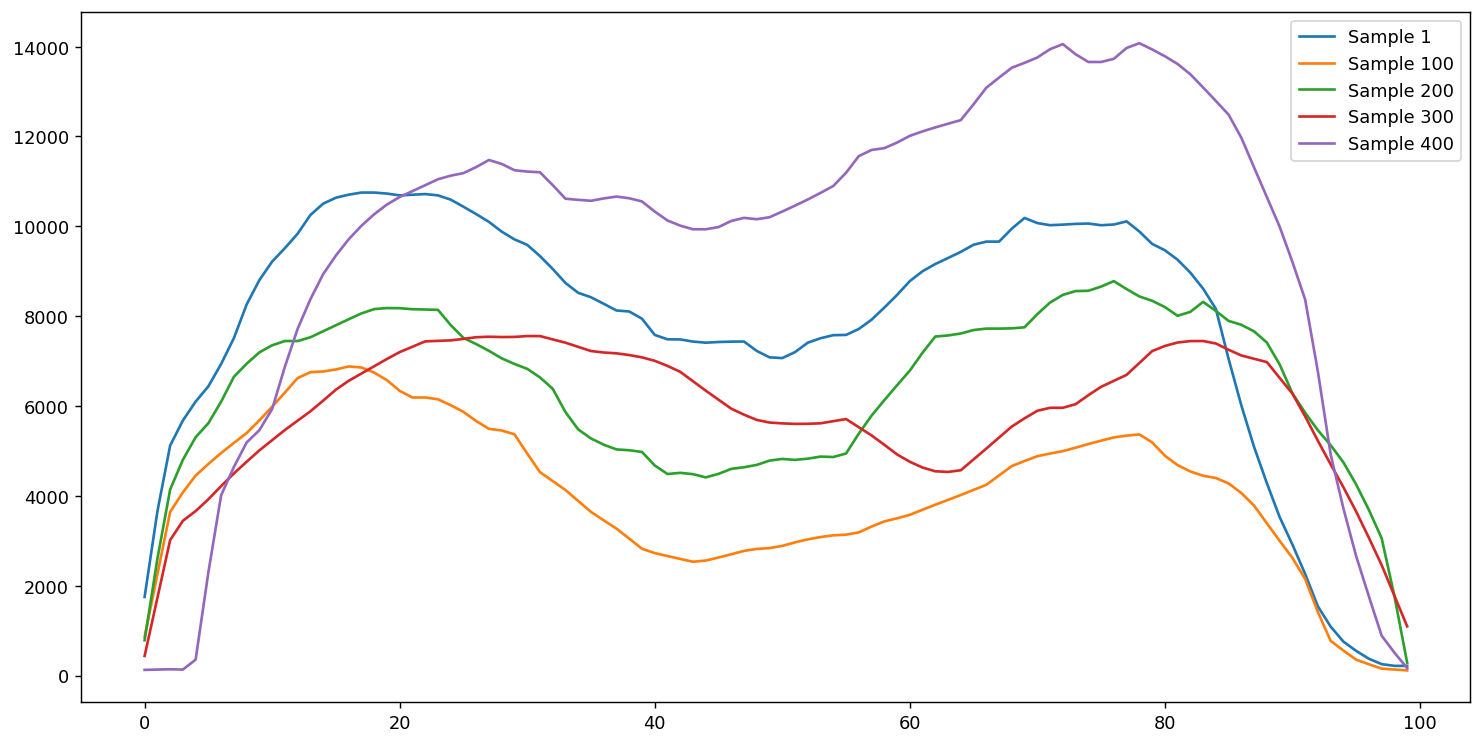
\includegraphics[width=0.9\textwidth]{figures/project/df_sum.png}
         \caption{The average pressure in each frame}
         \label{fig:extracted_features_sum}
     \end{subfigure}
     \vfill
     \begin{subfigure}[b]{0.5\textwidth}
         \centering
         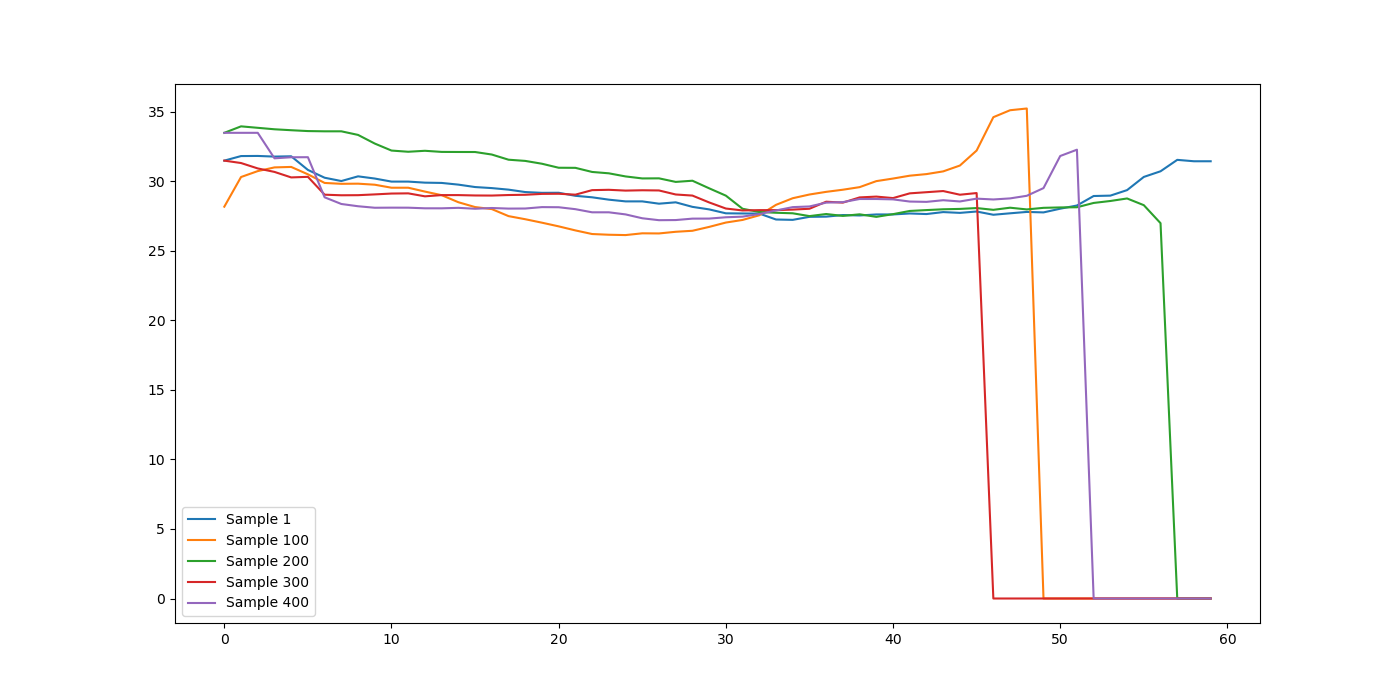
\includegraphics[width=0.9\textwidth]{figures/project/df_xCe.png}
         \caption{The x position in the center of pressure (COP) in each frame}
         \label{fig:extracted_features_xCe}
     \end{subfigure}
     \hfill
     \begin{subfigure}[b]{0.5\textwidth}
         \centering
         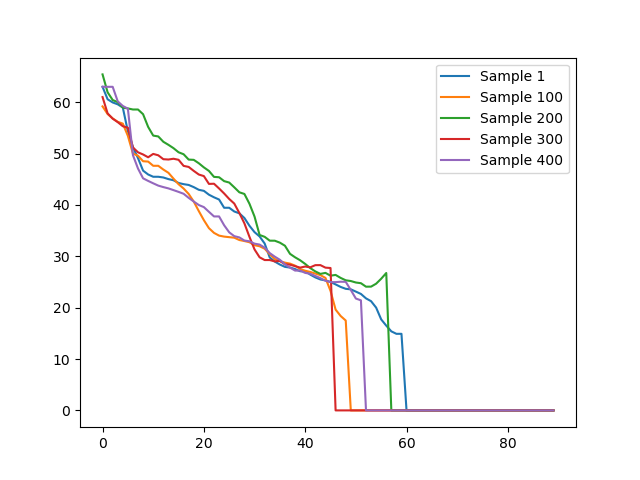
\includegraphics[width=0.9\textwidth]{manuscript/src/figures/project/df_yCe.png}
         \caption{The y position in the center of pressure (COP) in each frame}
         \label{fig:extracted_features_yCe}
     \end{subfigure} 
        \caption{The time series extracted from the Stepscan dataset based on four spatial features. The horizontal axis indicates the frame number.*******What is "each frame" in this context?  How does this related to gait/strides?  Be clear. }
        \label{fig:extracted_features}
\end{figure}






    \section{Literature Review}

%\subsection{The subsection also appears in the bookmarks}
DARPA, the Defense Advanced Research Projects Agency of the USA, started to research gait recognition by vision data in the early 2000s \cite{Connor2018BiometricFeatures}. Besides vision data \cite{Chen2006GaitModel}, some studies have instead used accelerometry from smartphones \cite{Mantyjarvi2005IdentifyingAccelerometers}, audio \cite{Geiger2013Gait-basedFeatures}, and underfoot pressures data \cite{Nakajima2000Footprint-BasedRecognition}. 







Addlesee in \cite{Addlesee1997TheFloor} used a new sensor (Active floor) for the first investigations into footprint recognition. This sensor was a square carpet tile maintained at the corners by some load cells and supplied the \gls{grf}. Orr and Abowd \cite{Orr2000TheTracking} extracted ten temporal features from the \gls{grf} curve. 

Moustakidis et al. \cite{Moustakidis2008SubjectSignals} extracted temporal features from the wavelet decomposition of \gls{grf} and then applied a kernel-based support vector machine. These studies have limitations in terms of the small sample sizes used for classification (e.g., 15 \cite{Orr2000TheTracking}, 10 \cite{Moustakidis2008SubjectSignals}, and 15 \cite{MiddletonARecognition}), and moderate classification rates ($CR < 90\%$).

Pataky in \cite{Pataky2012GaitIndividuals} could achieve a 99.6\% classification rate in a 104-participant dataset. This result was based on spatial alignment and automated dimensionality reduction. He used a template image that was made in \cite{Pataky2011AnEvaluation}. Pataky named this template the Munster-104 template.

In 2015, Cantoral-Ceballos \cite{Cantoral-Ceballos2015IntelligentEnvironments} introduced an intelligent carpet system. This carpet system (iMAGiMAT) worked based on the deformation of 116 distributed \gls{pof}. So that applying pressure to this system would change the intensity of the transmitted light. Thus the nature of the output of this sensor is time-series data.
 
Costilla-Reyes et al. \cite{Costilla-Reyes2016TemporalSystem} extracted five features directly from raw data of the iMAGiMAT sensor. These features were spatial Average (SA), standard deviation (SD), adjacent mean (AM), cumulative sum (CS), and cumulative product (CP).
They implemented 14 various machine learning methods for classification. The best result belonged to the Random Forest model with a validation score of $90.84 \pm 2.46\%$. 

Later, in \cite{Costilla-Reyes2018DeepSensors} they used an end-to-end convolutional neural network to extract Spatio-temporal features automatically. This technique increased their score by about 7 percent.

%Barandas et al. in \cite{Barandas2020TSFEL:Library} introduced a Python package entitled Time Series Feature Extraction Library (TSFEL). This Python package could compute more than 60 different features from the time-series data.


    \section{Features Extraction and Classifiers}

In this section, we describe algorithms along with their results. These are including Features Extraction and Selection, hyper-parameters of the classifier, and evaluation methodology. Afterward, the results are reported.

\subsection{Features Extraction and Selection}

As we mentioned before, our goal is to develop a classification model. For this classification task, we use about $34$ features in four categories. These feature sets are explained briefly here, and more details about them can be found in Appendix A.

After extracting features from each time series, some of Low variance and high-correlated features were eliminated. Feature selection causes the complexity of the model to reduce. Ten percent of handcraft features held out for testing our classifier, and others were divided into 10-fold cross-validation for evaluation and training. 

To have equally balanced classes in the test set and cross-validation set, the methods Stratified and StratifiedKFold were used. As a result, all subjects engaged in the test result. %for extracting features from each time series, we need to consider a windows that size with over  Each group of features implemented on a size for extracting features from each time series, we need to consider a windows that  
 
\subsubsection{Temporal Features}

The first set of features extracted was temporal features. In this set, we focused on features that related to the time axis. Features like Entropy, Absolute energy, Centroid, Area under the curve fall into this group. 

\subsubsection{Statistical Features}

Statistical information was another feature set that was extracted from the dataset. Min, Max, variance, and standard deviation were some of the statistical features. The total number of features in this group is about 10 for each time series.  

\subsubsection{Spectral Features}

In the third category, both FFT and wavelet transform were used to extract spectral information from the dataset. Not only the time complexity but also the number of features were more than two other feature sets. 
Max power spectrum, Maximum frequency, Spectral centroid, Wavelet energy, and FFT mean coefficient were spectral features extracted from the dataset.

\subsubsection{\Gls{AR} coefficients}

The final set of features in this research was the coefficients of \gls{AR}. In this set, the first-order differencing used to make our data stationary. Then based on significant lag on \gls{PACF}, the order of the model  was selected. This approach extracted two features for each time-series signal.

\subsection{Machine learning algorithms}

These time-series features fed to four different types of machine learning models with tuned hyper-parameters. The hyper-parameters tuning was implemented by grid search and performance evaluation with a 10  StratifiedKFold cross-validation. Table \ref{tab:1_ML} shows these models along with their best-tuned hyper-parameters.

\subsection{Results Progress}

Results of four different machine learning algorithms in several types of features are shown in table \ref{tab:1_ML}. For comparing algorithms, the accuracy metric was used. 
 
The LDA classifier’s best performance was a 69.2\% accuracy, as shown in table \ref{tab:1_ML}. This result comes from classifying the combination of all features. 
The kNN algorithm had similar performance on all kinds of features except \gls{AR} features. All algorithms had the worst results on this group of features.

The SVM performed best with the mixture of all features, at 56\% accuracy (see table \ref{tab:1_ML}). All other feature subsets achieved lower than this amount. The worst performance for all these classifiers belonged to the random forest classifier with about 30\%.

\begin{center}
	\begin{table*}[!t]
	\caption{Machine learning models along with its best-tuned hyper-parameters.}
	\label{tab:1_ML}
	\hspace{-1em}
%	\setlength\extrarowheight{-2pt}
	{\small
\begin{tabular}{lllr}
\toprule
Classifier & $Features^{*}$ & Hyper-parameter(s) & Accuraccy \\
\midrule
LDA & All & {'n\_components': 10 }& 69.28\% \\
kNN & All & {'n\_neighbors': 9, 'metric': manhattan,'weights': distance }& 42.85\% \\
SVM & All & {'kernel': rbf, 'decision\_function\_shape': ovr, 'C': 1000, 'gamma': 0.0001 }& 60.00\%                 \\
$RFC^{**}$ & All & {'criterion': entropy, 'max\_depth': 11 }& 28.57\% \\ \hline



LDA & temporal & {'n\_components': 10 }& 47.43\%   \\
kNN & temporal & {'n\_neighbors': 21, 'metric': manhattan,'weights': distance}& 34.29\%    \\
SVM & temporal & {'kernel': rbf, 'decision\_function\_shape': ovr, 'C': 10, 'gamma': 0.01}& 46.29\%   \\
RFC & temporal & {'criterion': entropy, 'max\_depth': 9 }& 28.57\%     \\ \hline




LDA & statistical & {'n\_components': 10 }& 48.00\% \\
kNN & statistical & {'n\_neighbors': 15, 'metric': manhattan,'weights': distance }& 36.57\%               \\
SVM & statistical & {'kernel': linear, 'decision\_function\_shape': ovr, 'C': 10, 'gamma': 1 }& 43.43\% \\
RFC & statistical & {'criterion': gini, 'max\_depth': 23 }& 26.86\%     \\ \hline


 
 
 
 LDA & spectral & {'n\_components': 10 }& 57.71\%               \\
kNN & spectral & {'n\_neighbors': 7, 'metric': manhattan,'weights': distance }& 39.43\%               \\
SVM & spectral & {'kernel': linear, 'decision\_function\_shape': ovr, 'C': 0.1, 'gamma': 1 }& 48.57\%                 \\
RFC & spectral & {'criterion': entropy, 'max\_depth': 7 }& 32.00\%     \\ \hline


 
LDA & AR & {'n\_components': 1 }& 4.57\%               \\
kNN & AR & {'n\_neighbors': 21, 'metric': manhattan,'weights': distance }& 2.86\%               \\
SVM & AR & {'kernel': linear, 'decision\_function\_shape': ovr, 'C': 1000, 'gamma': 1 }& 8.00\%  \\
RFC & AR & {'criterion': gini, 'max\_depth': 19 }& 1.14\%     \\ 
\bottomrule
\multicolumn{3}{l}{ *   All features were standardized.}\\
\multicolumn{3}{l}{** Random Forest Classifier}
\end{tabular}
}

	\end{table*}
\end{center}
    
    \section{Discussion Progress}

The results indicate that spectral features are more powerful features for all machine learning algorithms. The reason behind this might be the number of features in this set. Based on table \ref{tab:Features_list}, there are about 300 features for this set, much more than two others.

Another feature that has a significant effect on the accuracy is inter stride distance. This feature increased the accuracy of LDA from 60\% to 69\%. This feature just added to all features. 
 
The results might suggest that using AR features are not significant impact on accuracy. The accuracy of LDA without these features reduced to 68.57\%. 

Since we used one window for extracting temporal and statistical features, these results are not reliable for the quality of these two sets. Furthermore, it should be taken into account that the times-series signals contained many zeros due to the fact that videos were not normalized in the time axis. Thus, these zeros could bring a negative impact on temporal and statistical features.




%The results do not fit with the theory that…
%The experiment provides a new insight into the relationship between…


%The data contributes a clearer understanding of…
%While previous research has focused on X, these results demonstrate that Y.
%The generalizability of the results is limited by…
%The reliability of this data is impacted by…
%The methodological choices were constrained by…
%It is beyond the scope of this study to…






    %\section{Constraints}
%The constraints in this project could fall into two groups. The first constraint is related to the limitation on laboratory conditions \cite{Connor2018BiometricFeatures}. In real-world circumstances, many situations such as walking speed, clothing, footwear, and load carriage could affect our results, whereas our datasets could cover some of these real-world conditions. For example, except for the walking speed and footwear, both datasets do not have useful information for other real-world situations. Consequently, our results are optimistically biased. Table \ref{tab:1_vul} indicates some inhibiting factors. 

%Another significant limitation in the Stepscan dataset is the lack of relative footprint location. The dataset included only aligned and segmented footprint images. The location of samples concerning each other is unknown. This information could play a significant role in predicting the location of future footsteps. 

%\begin{center}
%	\begin{table}[!t]
%	\caption{Some inhibiting factors in gait recognition.}
%	\label{tab:1_vul}
%	\hspace{3em}
%	\setlength\extrarowheight{-2pt}
%	\begin{tabular}{rl}
\toprule
    &  Inhibit Factors \\
\midrule
  1 & Footwear               \\
  2 & clothing               \\
  3 & Injury                 \\
  4 & Muscle development     \\
  5 & Fatigue                \\
  6 & Age                    \\
  7 & Load carriage          \\
  8 & Walking speed          \\
  
\bottomrule
\end{tabular}


%	\end{table}
%\end{center}
 

\section{Remaining Work}

In recent years, improvements in the computational process of computers and other benefits of \gls{dnn} have caused many researchers (like \cite{IsmailFawaz2019DeepReview} and \cite{Costilla-Reyes2018DeepSensors}) to move towards \gls{dnn} for the classification of time series data. Therefore, these algorithms will be reviewed in a later stage of this project.

Because the entire time series were considered for extracting features, we have had one value for each attribute. For instance, while local maximums could be good features, the algorithm returned only the global maximum as a Max feature. We could slide a window on the signal to extract handcrafted features. It causes only a part of the data to consider in each moment. In other words, because each data includes several stages of the walking cycle, features should be extracted according to these periods.   

Moreover, cropping the heel or toe area in each video could separate features based on the walking stages (pressure area). By this means, each video will be divided into N sub-area, and then for each region, we reconstruct time-series signals and extract features. As a result, these features belong only to that area or stage of walking.

%Due to using the aligned video, we could consider some pixels over time as 2D signals. Although our features space increased rapidly, we could put a threshold on variance and energy of time-series signals for controlling features space. 

In this research, regardless of eliminating high-correlated and low variance features, we should use a more complex feature selection algorithm to eliminated irrelevant and redundant ones. This reduction might increase the accuracy.

%In addition, it had better to split the dataset into left and right footprints for exploring the effects of extracted features on classifier accuracy. 
 




%    \newpage
%    \section{CNN}



\paragraph{Functionality} The Elsevier article class is based on the standard article class and supports almost all of the functionality of that class. In addition, it features commands and options to format the
\begin{itemize}%\begin{enumerate}[(1)]
\item document style
\item baselineskip
\end{itemize}



\begin{figure}
    \centering
    \begin{minipage}[b]{.5\textwidth}
        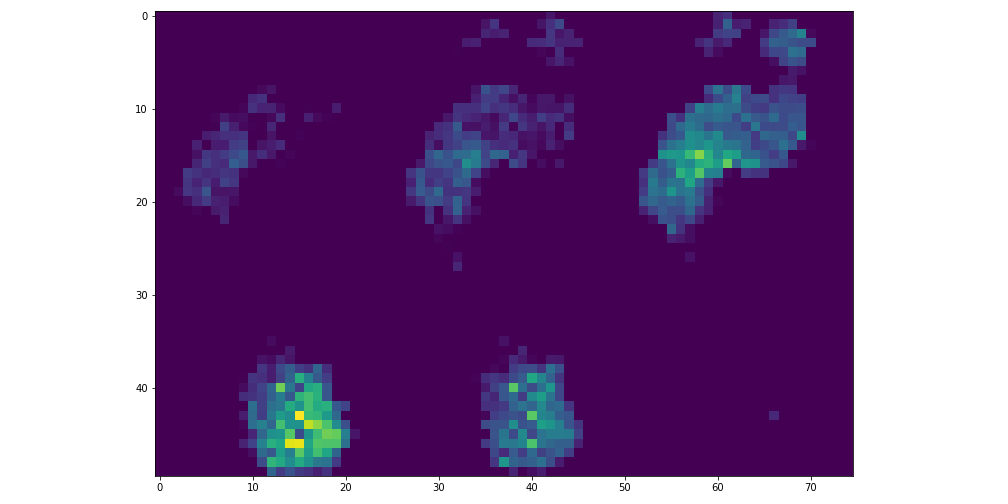
\includegraphics[width=\textwidth]{figures/project/frame1.png}
    \end{minipage}
    \caption{sample image.}
    \label{fig:Stepscan_dataset}
\end{figure}


Here are two sample references: \cite{SKazemii/EE6563}.
    
%\section*{\#TODO:}
%\begin{enumerate}[(1)]
%\item should normalized
%\item You want to focus on temporal information, and how it will help.\\

%\item Aren't they both time-series?  Are you just referring to the method that they are stored?   An array of images over time (video) is still a time series.\\ 
%\item You should show them as separate frames; how can you show the temporal aspects better?\\
%\item But these are just spatial features plotted over time? What are the proposed temporal features? \\
%\item Are you only thinking about within cycle information?  What about inter-stride information?  (for example, inter-stride variability is a well known gait feature).\\
%\item Have you explored relationships between pixels/features over time?
%\item Does Costilla-Reye's work deserve a bit more discussion?  Is that the current state-of-the-art?
 

%\item Focus on what is important; where is the temporal information going to come from?  Time series of spatial information?  Temporal features?  Temporal algorithms applied to spatial features?  Are the features only within stride, or are your features going to be inter-stride?


%\item Is this the main benefit? (No)


%\end{enumerate}    
    
%\nolinenumbers
\bibliography{references}
 

\newpage
%\pagenumbering{gobble}
%\begin{landscape}
%\newgeometry{left=1cm}
\onecolumn
\appendix
\label{appendix:1}
\section{List of features}
The list of features from several categories used in this project (Table \ref{tab:Features_list}):

{%\small
%\tablinesep=2ex\tabcolsep=10pt

\hspace{-6cm}
\begin{tabularx}{\linewidth}{@{}rlccc@{}}
\caption{list of features} \\
\label{tab:Features_list}\\
\toprule
  \#  &  Features Name & {Categories Name } & \# features & description\\
\midrule
\endfirsthead
\toprule
  \#  &  Features Name & {Categories Name } & \# features & description\\
\midrule
\endhead
\midrule
\multicolumn{4}{r}{\footnotesize( To be continued)}
\endfoot
\bottomrule
\endlastfoot

%  1 & ECDF              & Statistical  & A\\
%  2 & ECDF Percentile      & Statistical  & A         \\
%  3 & ECDF Percentile Count & Statistical  & A\\
  1 & Histogram    & Statistical  & 10 & 10-bin Histogram \\
%  5 & Interquartile range               & Statistical  & A \\
%  6 & Kurtosis                   & Statistical  & A \\
  2 & Max         & Statistical  & 1 & max(s)\\
  3 & Mean         & Statistical   & 1 & mean(s)\\
  4 & Mean absolute deviation         & Statistical   & 1 & ${\Sigma_{i=1}^{N} |S_i^2 - mean(s)|}/{N}$\\
  5 & Median         & Statistical   & 1 & median(s)\\
  6 & Median abs deviation         & Statistical   & 1 & $median(|s - median(s)|)$\\
  7 & Min         & Statistical   & 1  & min(s)\\
  8 & Root mean square         & Statistical   & 1 & $\sqrt{{\Sigma_{i=1}^{N} S_i^2}/{N}}$\\
  %9 & Skewness         & Statistical   & A\\
  9 & Standard deviation         & Statistical   & 1 & $\sqrt{var}$\\
  10 & Variance         & Statistical   & 1 & $mean(|s - mean(s)|^2)$\\ \hline
   11 & AR coefficients & \Gls{AR} & 8 & -\\\hline
  12 & Absolute energy         & Temporal  & 1 & ${\Sigma_{i=0}^{N} S_i^2 }$ \\%& The absolute energy of the signal.\\
  13 & Area under the curve         & Temporal   & 1& ${\Sigma_{i=0}^{N} (t_i - t_{i-1}) \times (s_i + s_{i-1})/2 }$\\ %& Computes the area under the curve of the signal.\\
  %19 & Autocorrelation         & Temporal   & -1\\
  14 & Centroid         & Temporal   & 1 & ${\Sigma_{i=0}^{N} (t_i \times s_{i}^2) / \Sigma_{i=0}^{N} s_{i}^2}$\\%& Computes the centroid along the time axis\\
  15 & Entropy         & Temporal   & 1 & ${- \Sigma P(x) log_2 P(x)}$\\%& Computes the Shannon entropy of the signal\\
  16 & Mean absolute diff         & Temporal   & 1 & $mean(|diff(s)|)$\\ %& Computes mean absolute differences of the signal\\
  17 & Mean diff         & Temporal   & 1 & $mean(diff(s))$\\%& Computes mean of differences of the signal.\\
  18 & Median absolute diff         & Temporal   & 1 & $median(|diff(s)|)$\\%& Computes median absolute differences of the signal.\\
  19 & Median diff         & Temporal   & 1 & $median(diff(s))$\\%& Computes median of differences of the signal. \\
  %20 & Negative turning points         & Temporal   & 1\\ %& Computes number of negative turning points of the signal.\\
  %28 & Neighbourhood peaks         & Temporal   & 1 & Computes the number of peaks from a neighbourhood of the signal.\\
  %21 & Positive turning points         & Temporal   & 1 \\%& Computes number of positive turning points of the signal. \\
  %30 & Signal distance         & Temporal   & -1 & \\
  20 & Slope         & Temporal   & 1 & fitting a line and returning the slope\\\hline%& by fitting a linear equation to the observed data.\\
  %32 & Sum absolute diff         & Temporal   & A\\
  %33 & Total energy         & Temporal   & A\\
  %34 & Zero crossing rate         & Temporal   & -1\\
  %35 & Neighbourhood peaks         & Temporal   & A\\
  21 & FFT mean coefficient         & Spectral   & 256 & mean(fft(s)) \\
  %37 & Fundamental frequency         & Spectral   & A\\
  %38 & Human range energy         & Spectral   & A\\
  %39 & LPCC         & Spectral   & A\\
  %40 & MFCC         & Spectral   & A\\
  22 & Max power spectrum         & Spectral   & 1 & -\\%$computing~the~ maximum~power~spectrum~density.$\\
  23 & Maximum frequency         & Spectral   & 1 & -\\
  24 & Median frequency         & Spectral   & 1 & -\\
  %44 & Power bandwidth         & Spectral   & A\\
  25 & Spectral centroid         & Spectral   & 1 & -\\
  %46 & Spectral decrease         & Spectral   & A\\
  %47 & Spectral distance         & Spectral   & A\\
  26 & Spectral entropy         & Spectral   & 1 & -\\
  %49 & Spectral kurtosis         & Spectral   & A\\
  %50 & Spectral turning points         & Spectral   & A\\
  %51 & Spectral roll-off         & Spectral   & A\\
  %52 & Spectral roll-on         & Spectral   & A\\
  %53 & Spectral skewness         & Spectral   & A\\
  %54 & Spectral slope         & Spectral   & A\\
  %55 & Spectral spread         & Spectral   & A\\
  %56 & Spectral variation         & Spectral   & A\\
  27 & Wavelet abs mean         & Spectral   & 10 & $|mean(wavelet(s))|$\\
  28 & Wavelet energy         & Spectral   & 10 & -\\%$computing~ CWT~ energy~ of~ each ~wavelet ~scale.$\\
  29 & Wavelet stand deviation         & Spectral   & 10& $|std(wavelet(s))|$\\
  30 & Wavelet entropy         & Spectral   & 1 & -\\%$computing~ CWT~ entropy~ of~ the~ signal.$\\
  31 & Wavelet variance         & Spectral   & 10 & $|var(wavelet(s))|$\\ \hline
  32 & Inter stride         & Temporal   & 1\\ \hline
\multicolumn{3}{r}{The total number of features} & 340\\
\end{tabularx}\hspace*{-4cm}
}



%\end{landscape}
\end{document}